\documentclass[11pt]{article}
%\renewcommand{\thesection}{\Roman{section}}
\setlength{\parindent}{0in}
\setlength{\parskip}{\baselineskip}
\usepackage{times}
\usepackage{graphicx}
\usepackage[pdftex]{hyperref}
\topmargin -5pt
\renewcommand{\leftmargini}{0pt}
\oddsidemargin 0.3in \textwidth 6.2in
\headheight 0pt
\headsep 0pt
\textheight 48\baselineskip
\begin{document}

\Large
DEGAS 2 \\
\ \\
\normalsize

\begin{centering}
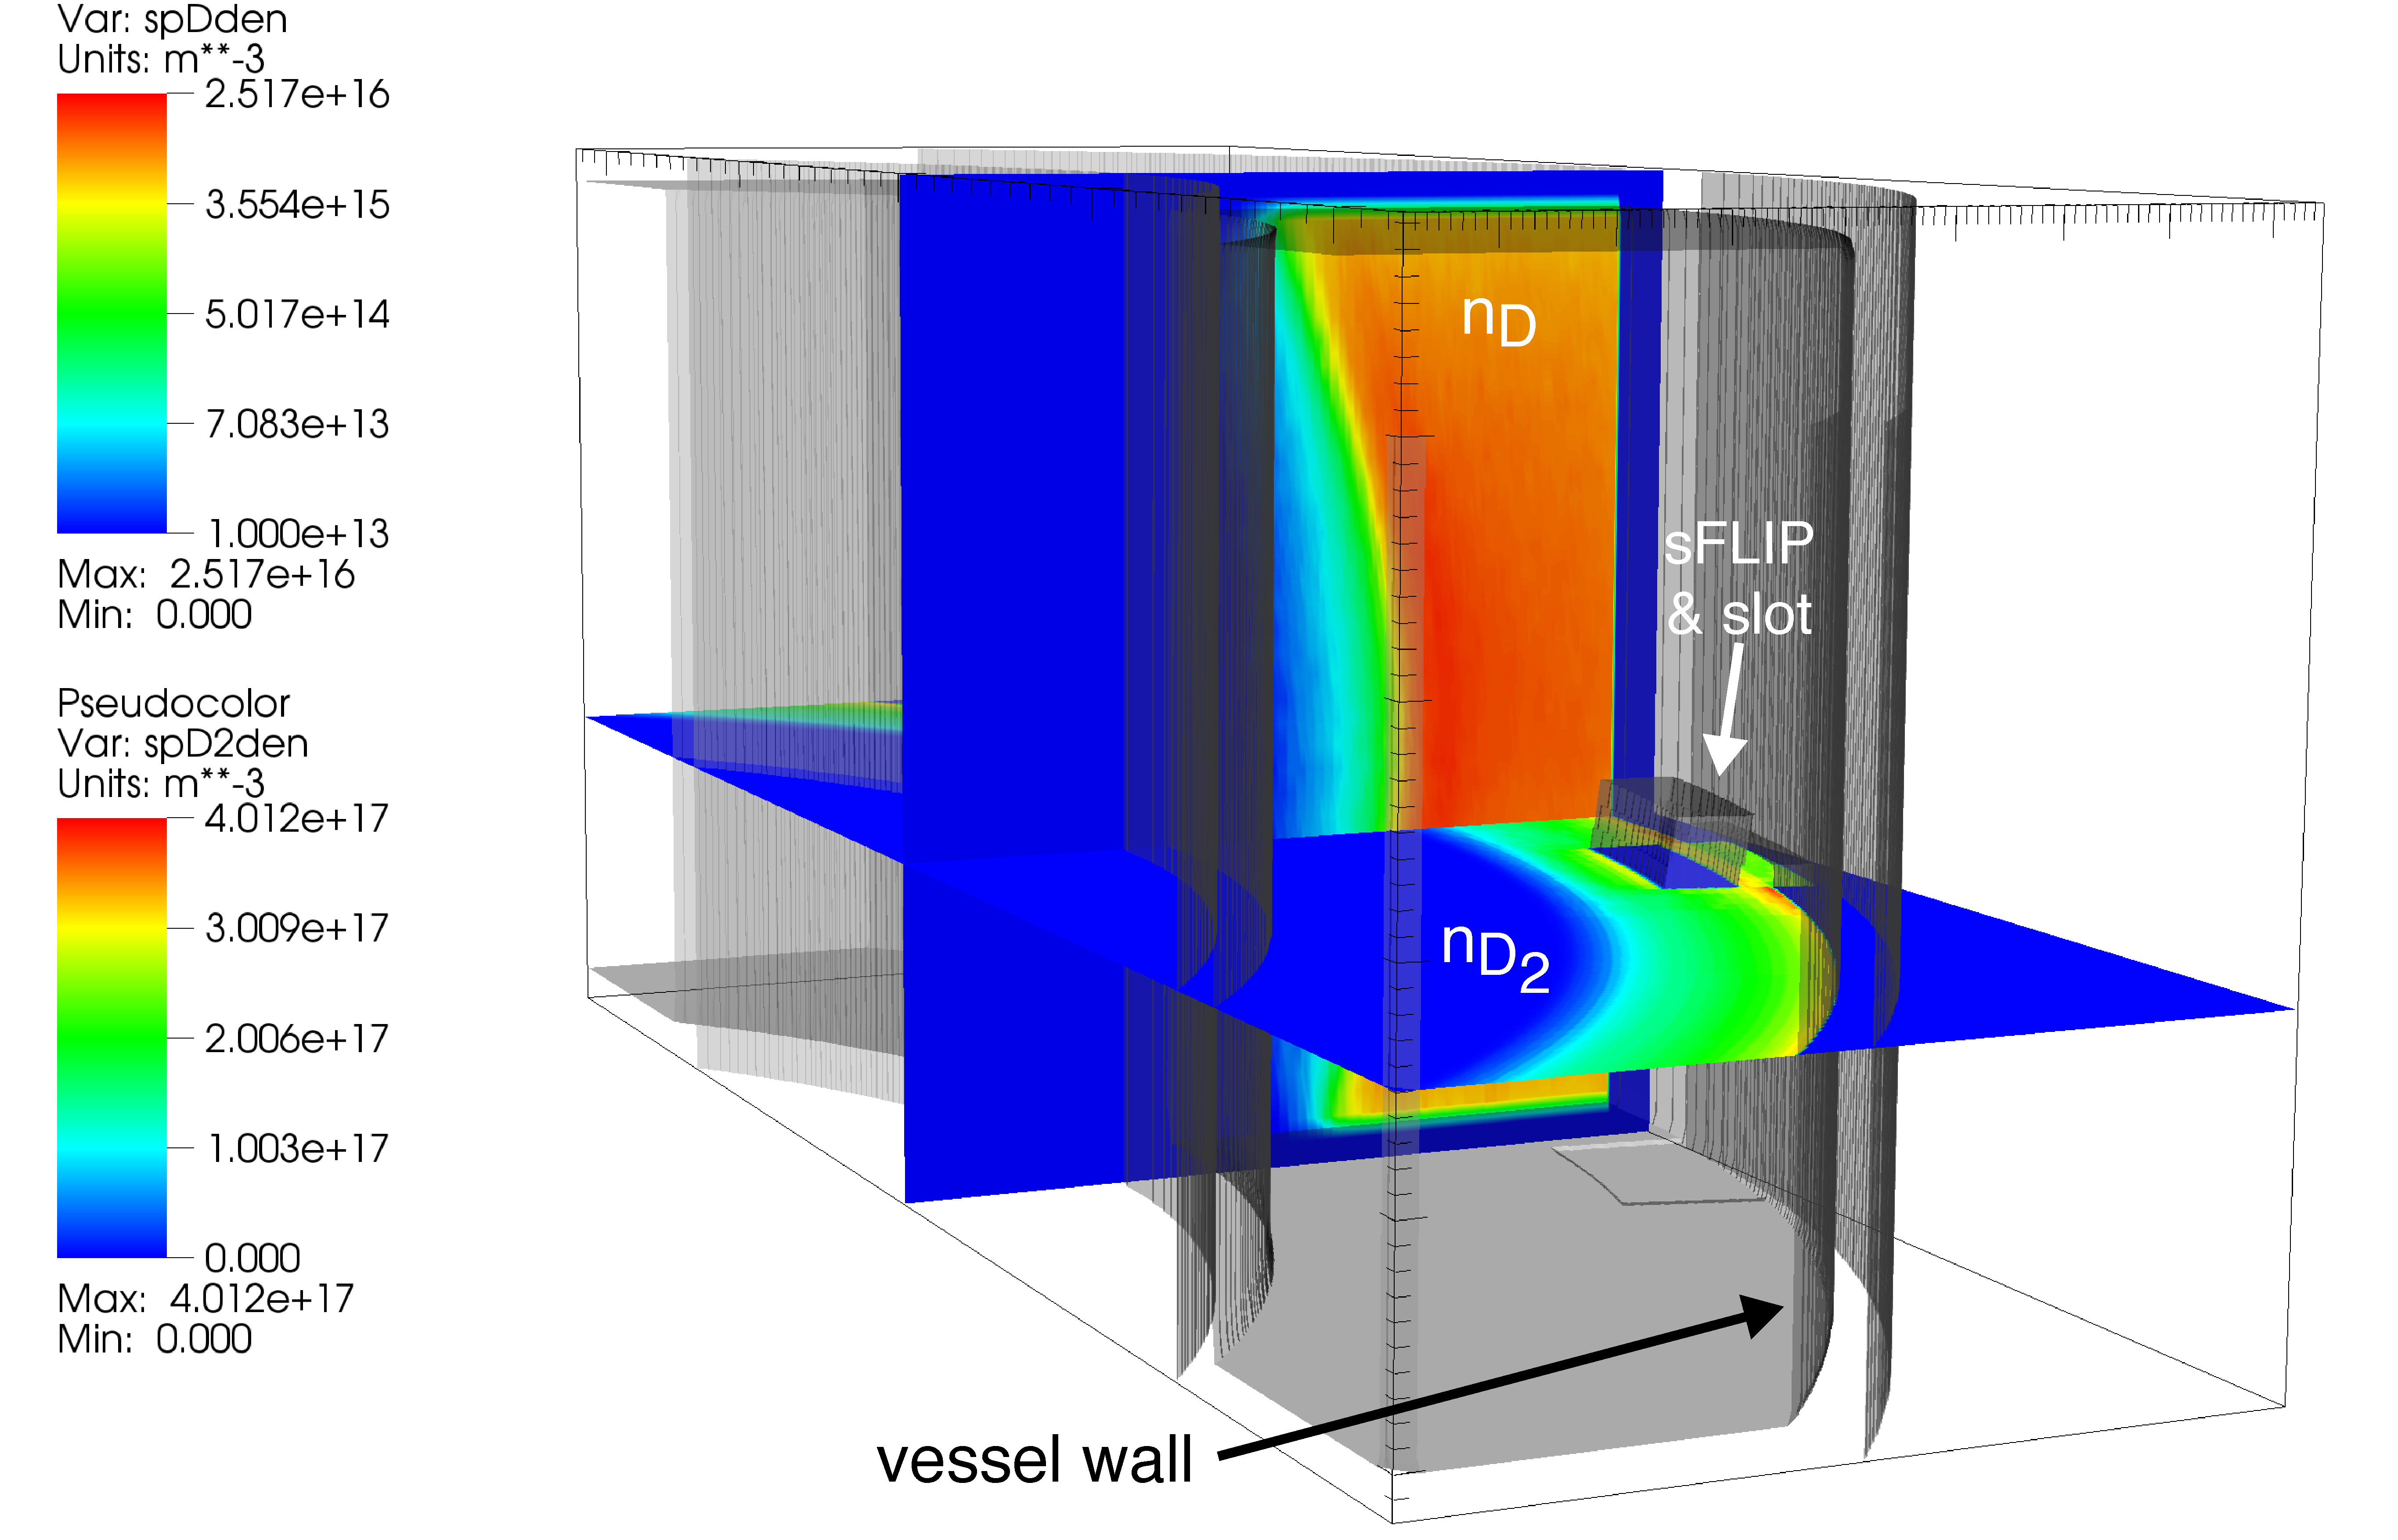
\includegraphics[width=12.0cm]{D_D2_den_3D} \\
{\bf Slices through the three-dimensional atomic (vertical)
and molecular (horizontal) deuterium profiles in a
simulation of data from the NSTX Edge Neutral Density
Diagnostic.}
\end{centering}

Neutral atoms and molecules in fusion plasmas
are of interest for multiple reasons.  First, neutral
particles are produced via the interactions of the plasma
as it flows along open field lines to surrounding material
surfaces.  Unconfined by the magnetic field, the atoms and
molecules provide a channel for heat transport across the field
lines and also serve as a source of plasma particles via ionization.
Second, atoms that penetrate well past the last closed 
flux surface can charge exchange with plasma ions to 
generate high energy neutrals that can strike the 
vacuum vessel wall,
sputtering impurities into the plasma and 
possibly damaging the wall.  Third, the most common means of fueling
plasmas is with an external puff of gas.  Finally, the light emitted
by the neutral atoms and molecules in all of 
the above processes can be
monitored and used as the basis for diagnostics.

Kinetic models of neutral particle transport are
based 
on the Boltzmann equation. For the simple case of a 
single ``background'' species and a single binary collision
process, this is:  
\begin{eqnarray*}
\frac{\partial f({\bf r}, {\bf v}, t)}{\partial t}
& + & {\bf v} \cdot \nabla_{\bf r} f({\bf r}, {\bf v}, t) \\
& = & \int d{\bf v}^{\prime} \, d{\bf V}^{\prime} \, d{\bf V} \sigma( {\bf v}^{\prime}, {\bf V}^{\prime};
{\bf v}, {\bf V}) | {\bf v}^{\prime} - {\bf V}^{\prime} | f({\bf v}^{\prime}) f_{b}({\bf V}^{\prime}) \\
& - & \int d{\bf v}^{\prime} \, d{\bf V}^{\prime} \, d{\bf V} \sigma( {\bf v}, {\bf V};
{\bf v}^{\prime}, {\bf V^{\prime}}) | {\bf v} - {\bf V} | f({\bf v}) f_{b}({\bf V}),
\label{BE}
\end{eqnarray*}
% Essential references for the equations are Kotov's thesis (the Juelich report?)
% and Case and Zweifel.  After going back to it, the Eirene manual is probably
% better than Kotov's thesis.
where $f({\bf r}, {\bf v}, t)$ and $f_{b}({\bf r}, {\bf V}, t)$ are the neutral 
and background distribution functions, respectively,
and
$\sigma$ is the differential
cross section for the collision process.  The first (second) 
integral on the right-hand
side represents scattering into (out of) the velocity $v$. 

DEGAS 2 \cite{Stot94}, like its predecessor, DEGAS \cite{Heif82}, uses 
the Monte Carlo approach to integrating the Boltzmann
equation, allowing the treatment of complex geometries, atomic
physics, and wall interactions.
DEGAS 2 is written in a ``macro-enhanced''
version of FORTRAN via the FWEB library, providing an object oriented capability
and simplifying tedious tasks, such as dynamic memory allocation and the reading
and written of self-describing binary files.  As a result, the code is
extremely flexible and can be readily adapted to problems seemingly far removed
from tokamak divertor physics, e.g., its use in simulating
the diffusive evaporation of lithium in NSTX \cite{Stot2011} and LTX \cite{Schm2013}.

DEGAS 2 has been extensively verified, as is documented in its 
User's Manual \cite{D2UM}.
Experimental validation has been largely centered on the Gas Puff Imaging (GPI)
technique for visualizing plasma turbulence in the tokamak edge.
The validation against
deuterium gas puff data from NSTX is described in the paper by 
B. Cao et al. \cite{Cao2013}  
Analogous work with both deuterium and helium has been carried out on
Alcator C-Mod.  A related application of DEGAS 2 is in the interpretation of data from
the Edge Neutral Density Diagnostic on NSTX \cite{Stot2015} and NSTX-U.  DEGAS 2
has been applied to many other devices, including JT-60U \cite{Take2002},
ADITYA \cite{Dey2017}, and FRC experiments at Tri-Alpha Energy \cite{Gran2018}.
% http://adsabs.harvard.edu/abs/2016APS..DPPC10077G
%  http://meetings.aps.org/Meeting/DPP18/Session/PP11.83

Neutral transport codes are frequently coupled to plasma simulation
codes to allow a self-consistent plasma-neutral solution to be 
computed.
Initially,
DEGAS 2 was coupled to UEDGE \cite{Stot2000}.
More
recently, DEGAS 2 has been coupled to the 
drift-kinetic XGC0 \cite{Stot2013}, and has been
used in the development and testing of the simplified built-in neutral transport
module in XGC1 \cite{Stot2017}.   A related project is a DEGAS 2-based synthetic
GPI diagnostic for XGC1 \cite{Stot2019}.

\begin{thebibliography}{10}
\expandafter\ifx\csname url\endcsname\relax
  \def\url#1{\texttt{#1}}\fi
\expandafter\ifx\csname urlprefix\endcsname\relax\def\urlprefix{URL }\fi
\expandafter\ifx\csname href\endcsname\relax
  \def\href#1#2{#2} \def\path#1{#1}\fi

\bibitem{Stot94} D.~P. Stotler and C.~F.~F. Karney, 
\href{http://dx.doi.org/10.1002/ctpp.2150340246}{Contrib. Plasma Phys. {\bf 34}, 392 (1994)}

\bibitem{Heif82}
D. Heifetz, D. Post, M. Petravic, J. Weisheit, and 
G. Bateman, 
\href{https://doi.org/10.1016/0021-9991(82)90017-1}{J. Comp. Phys. {\bf 46}, 309 (1982)}

\bibitem{Stot2011}
D.~P. Stotler et al., \href{http://dx.doi.org/10.1016/j.jnucmat.2010.11.070}{J. Nucl. 
Mater. {\bf 415}, S1058 (2011)}

\bibitem{Schm2013}
J.~C. Schmitt et al., 
\href{http://dx.doi.org/10.1016/j.jnucmat.2013.01.241}{J. Nucl. Mater. {\bf 438}, S1096 (2013)}

\bibitem{D2UM}
\href{https://w3.pppl.gov/degas2/}{DEGAS 2 Home Page}

\bibitem{Cao2013}
B. Cao et al.,, \href{https://doi.org/10.13182/FST13-A17044}{Fusion Sci. Tech.
{\bf 64}, 29 (2013)}

\bibitem{Stot2015}
D.~P. Stotler et al., \href{http://dx.doi.org/10.1063/1.4928372}{Phys. Plasmas {\bf 22},
082506 (2015)}

\bibitem{Take2002}
H. Takenaga et al., \href{https://doi.org/10.1088/0029-5515/41/12/305}{Nucl. Fusion
{\bf 41}, 1777 (2001)}

\bibitem{Dey2017}
R. Dey et al., \href{https://doi.org/10.1088/1741-4326/aa739c}{Nucl. Fusion
{\bf 57}, 086003 (2017)}

\bibitem{Gran2018}
E.~M. Granstedt et al., \href{http://meetings.aps.org/Meeting/DPP18/Session/PP11.83}{Presented
at 60th Annual Meeting of the APS Division of Plasma Physics}

\bibitem{Stot2000}
D.~P. Stotler et al., \href{https://doi.org/10.1002/1521-3986(200006)40:3/4<221::AID-CTPP221>3.0.CO;2-L}{Contrib.
Plasma Phys. {\bf 40}, 221 (2000)}

\bibitem{Stot2013}
D.~P. Stotler et al., \href{http://dx.doi.org/10.1088/1749-4699/6/1/015006}{Comput.
Sci. Disc. {\bf 6}, 015006 (2013)}

\bibitem{Stot2017}
D.~P. Stotler et al., \href{https://doi.org/10.1088/1741-4326/aa7807}{Nucl. Fusion
{\bf 57}, 086028 (2017)}

\bibitem{Stot2019}
D.~P. Stotler et al., \href{https://psi2018.princeton.edu/}{Presented at the 23rd
International Conference on Plasma Surface Interactions in Controlled
Fusion Devices}












\end{thebibliography}  

\end{document}

